\documentclass[11pt]{article}
\usepackage{titling}
\usepackage[english]{babel}
\usepackage[margin=0.6in]{geometry} % Page Dimension

%%%%%%%%%%%%%%%%%%%%%%%%%%%%%%%%%%%%%%%%%%
%                PACKAGES                %  
%%%%%%%%%%%%%%%%%%%%%%%%%%%%%%%%%%%%%%%%%%

% Styling Choices
\setlength{\parskip}{\baselineskip}%

% Math
\usepackage{amsmath, amsthm, amssymb}
\usepackage[inline]{asymptote}
\usepackage{xcolor}
\usepackage{cancel}
\usepackage{tikz}
\usepackage{enumitem}
\usepackage[europeanresistors,americaninductors,americancurrents,siunitx]{circuitikz}

\newcommand{\thiscirc}[1]{
\texttt{#1} \hfill \begin{circuitikz} \draw
(0,0) node[ #1 ] {};%(2,0); 
\end{circuitikz} {\hspace{5mm}}}


\newcommand{\bipole}[1]{
\texttt{#1} \hfill \begin{circuitikz} \draw
(0,0) to[ #1 ] (2,0); 
\end{circuitikz} {\hspace{5mm}}}

% Allows for hyperlinking
\usepackage{hyperref}
\hypersetup{
    colorlinks=true,
    linkcolor=magenta,
}

% Blind Footnote
\newcommand\blfootnote[1]{%
  \makeatletter{\footnotetext{#1}\makeatother}
}

% Fancy Header
\usepackage{fancyhdr}
\pagestyle{fancy}
\lhead{Kalda Circuits}
\rhead{\thepage}

% Coloured Boxes
\usepackage{xcolor}
\definecolor{border}{HTML}{004D4D}
\definecolor{hard}{HTML}{ffccb3}
\definecolor{easy}{HTML}{b3e6b3}
\definecolor{normal}{HTML}{f2f2f2}

% Syntax: \colorboxed[<color model>]{<color specification>}{<math formula>}
\newcommand*{\colorboxed}{}
\def\colorboxed#1#{%
  \colorboxedAux{#1}%
}
\newcommand*{\colorboxedAux}[3]{%
  % #1: optional argument for color model
  % #2: color specification
  % #3: formula
  \begingroup
    \colorlet{cb@saved}{.}%
    \color#1{#2}%
    \boxed{%
      \color{cb@saved}%
      #3%
    }%
  \endgroup
}

% Setup Gray Solution Boxes
\usepackage[breakable,many]{tcolorbox}
\newtcolorbox[auto counter]{solution}[1]{
    enhanced, breakable,
    arc=0pt,
    % colback=default, % Background color
    colframe=white, % Border Color
    coltitle=black, % Title Color
    fonttitle=\bfseries,
    title=\fcolorbox{border}{#1}{\textcolor{border}{pr} \bfseries \textcolor{border}{\thetcbcounter}.},
    attach title to upper,
    after title={\ },
    segmentation style={dashed, gray},
}

% Title and front page
\title{Solutions to Problems in Electrical Circuits Handout by Jaan Kalda With detailed diagrams and walkthroughs}
% Author
\author{\textsc{Ashmit Dutta, QiLin Xue, Kushal Thaman, Arhaan Ahmad}}

\begin{document}
\usetikzlibrary{calc}
\begin{titlepage}
    \begin{center}
        \vspace*{1cm}
 
        \Huge
        \textbf{Solutions to Jaan Kalda's Problems in Electrical Circuits}
 
        \vspace{0.5cm}
        \LARGE
        \textbf{With detailed diagrams and walkthroughs}
        
        \vspace{0.1cm}
        Edition 1.2.1
        
        \vspace{1.2cm}
 
         Ashmit Dutta, QiLin Xue, Kushal Thaman, Rakshit
        \vspace{10mm}
        \vfill
        
        \Large
        Updated
        \today
 
    \end{center}
\end{titlepage}
\newpage
%%%%%%%%%%%
% Preface %
%%%%%%%%%%%
\section*{Preface}
\vspace{-5mm}
\indent Jaan Kalda's \href{https://www.ioc.ee/~kalda/ipho/}{handouts} are beloved by physics students both in for a quick challenge, to students preparing for international Olympiads. As of writing, the current \href{https://www.ioc.ee/~kalda/ipho/electricity-circuits.pdf}{circuits} handout (ver 1.2) has 111 unique problems and 52 main `ideas'.

This solutions manual came as a pilot project from the online community at \url{artofproblemsolving.com}. Although there were detailed hints provided, full solutions have never been written. The majority of the solutions seen here were written on a private forum given to those who wanted to participate in making solutions. In an amazing show of an online collaboration, students from around the world came together to discuss ideas and methods and created what we see today.

This project would not have been possible without the countless contributions from members of the community. Online usernames were used for those who did not wish to be named: 

\textit{Heramb Podar, Ameya Deshmukh, Viraj Jayam, Rakshit, dbs27, Anant Lunia, Jai, Sean Chen, Ayon Ghosh, Joshua S, Tarun Agarwal, c\_deng}
\subsection*{Structure of The Solutions Manual}
\vspace{-5mm}
Each chapter in this solutions manual will be directed towards a section given in Kalda's circuits handout. There are two major sections: circuits with resistors, batteries, ammeters, and voltmeters, and circuits including capacitors and inductances. If you are stuck on a problem, cannot make progress even with the hint, and come here for reference, look at only the start of the solution, then try again. Looking at the entire solution wastes the problem for you and ruins an opportunity for yourself to improve.

\subsection*{Contact Us}
\vspace{-5mm}
Despite editing, there is almost zero probability that there are \textit{no} mistakes inside this book. If there are any mistakes, you want to add a remark, have a unique solution, or know the source of a specific problem, then please contact us at \url{hello@physoly.tech}. The most current and updated version can be found on our website \url{physoly.tech}

Please feel free to contact us at the same email if you are confused on a solution. Chances are that many others will have the same question as you.

\newpage
\section{Circuits with Resistors, Batteries, Ammeters, and Voltmeters}
\vspace{-5mm}

\begin{solution}{normal}
Since the segments marked by the streaks are originally the same volume, the volume of each of the segments must remain constant. Therefore, we have $A_0a_0 = Aa$, so $A = \dfrac{A_0a_0}{a}$. We know the resistance $\Delta R$ of a small segment of length $\Delta \ell$ is given by:
$$\Delta R = \dfrac{\rho}{A_0a_0/a}\Delta \ell = \dfrac{\rho a}{A_0a_0}\Delta \ell .$$By considering infinitesimally small segments, our total resistance is given by
$$R = \dfrac{\rho}{A_0a_0}\int_0^4a \, d\ell.$$We can estimate this value off of the graph, there are approximately 10 large boxes (visible) under the curve, plus the 4 more that aren't shown corresponds to $0.014 m^2$. So we have
$$R \approx \dfrac{(1.0\times 10^{-6})(0.014 m^2)}{1.0\times 10^{-9}} = \boxed{14 \, \mathrm{\Omega}}$$Additionally, we can also avoid a lot of the guesswork by approximating the curve as a sinusoidal curve. We can read off the coordinates of the minimum and maximum separation to be $(0.75, 1.78)$ and $(3.05, 4.93)$, which gives:
$$a(\ell) = 1.58\cos(1.37\ell - 4.15) + 3.36$$We can integrate this to get:
$$\int_0^4 a \text{ d}\ell = 13.6 \approx 0.014 \text{ m}^2$$which agrees with the estimate.
\end{solution}
\begin{solution}{normal}
\textbf{Long Way:} We can set arbitrary values for the voltage $U$, and the resistance $R_1$, so we will pick $U=5 \text{ V}$ and $R_1=4\,\Omega$. From the relationship relating $R_1$ and $R_2$, we also have $R_2 = 1\,\Omega$. Initially, the two resistors are in series, so the current $I_0$ running through the entire circuit is:
$$U = I_0(R_1+R_2) \implies I_0 = \frac{U}{R_1+R_2} = 1 \text{ A}.$$After the lightbulb is added, the current increases to $I'=1.1 \text{ A}$. The resistor $R_2$ is now in parallel with the lamp, which has a resistance of $r$. We can determine the equivalent resistance $R'_\text{eff}$ of the circuit to be:
$$R'_\text{eff} = R_1 + \frac{rR_2}{r+R_2} = 4 + \frac{r}{1+r}$$Using Kirchoff's voltage loop rule on the equivalent circuit, we can determine the value for $r$ given our initial setup to be:
$$U - I'R'_\text{eff} = 0 \implies 5 = 1.1\left(4 + \frac{r}{1+r}\right) \implies r = 1.2\,\Omega$$We can then use Kirchoff's voltage loop rule again, but on the loop which contains the voltage source, $R_1$, and $r$, such that:
$$U - I'R_1 - I_\text{lamp}r = 0 \implies 5 - (1.1)(4) - I_\text{lamp}(1.2) = 0 \implies \boxed{I_\text{lamp} = 0.5\text{ A}}.$$
\tcbline
\textbf{Short Way:} Let $I_1$ be the current through $R_1$ and let $I_2$ be the current through $R_2$. We know that$$I_1R_1+I_2R_2=\text{constant} \implies \Delta I_1 R_1 + \Delta I_2 R_2 = 0$$so we can compare the initial and final state of the system. If $I_1$ increases by $0.1 \text{ A}$, then $I_2$ must decrease by $0.4\text{ A}$. However, by Kirchhoff's junction rule, the sum of the currents must be zero:
$$I_\text{in} = I_\text{out}$$Since $I_1$ is increasing by $0.1\text{ A}$ and $I_2$ is decreasing by $0.4 \text{ A}$, then in order for this to be valid, the current through the lamp must increase (from zero) to be $\boxed{I_\text{lamp} = 0.5\text{ A}}$.
\end{solution}
\begin{solution}{easy}
We first label the nodes, as the problem suggests:
\begin{center}
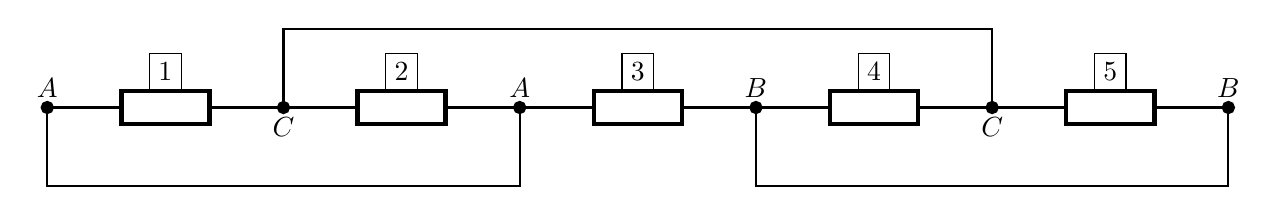
\begin{tikzpicture}[transform shape, thick]
size(2cm);
\ctikzset{bipoles/thickness=2}
\ctikzset{label/align = smart}
\coordinate  (A) at (0,0);
\coordinate  (C) at (3,0);
\coordinate  (A') at (6,0);
\coordinate  (B) at (9,0);
\coordinate  (C') at (12,0);
\coordinate  (B') at (15,0);

\draw[fill=black] (A) circle (2pt) node[above] {$A$};
\draw[fill=black] (A') circle (2pt) node[above] {$A$};
\draw[fill=black] (B) circle (2pt) node[above] {$B$};
\draw[fill=black] (B') circle (2pt) node[above] {$B$};
\draw[fill=black] (C) circle (2pt) node[below] {$C$};
\draw[fill=black] (C') circle (2pt) node[below] {$C$};

\draw (A) to [R, l=$\boxed{1}$] (C)
          to [R, l=$\boxed{2}$] (A')
          to [R, l=$\boxed{3}$] (B)
          to [R, l=$\boxed{4}$] (C')
          to [R, l=$\boxed{5}$] (B');
          
\draw (A) to ($(A) + (0, -1)$) to ($(A') + (0, -1)$) to (A');
\draw (B) to ($(B) + (0, -1)$) to ($(B') + (0, -1)$) to (B');
\draw (C) to ($(C) + (0, 1)$) to ($(C') + (0, 1)$) to (C');
\end{tikzpicture}
\end{center}
Here, the same labeled nodes have the same potential as they are connected with a wire. We can redraw this to be something more convincing by considering each node one at a time. Node $A$ is directly connected to resistors $\boxed{1}$, $\boxed{2}$, and $\boxed{3}$. Node $C$ is connected directly to everything except resistor $\boxed{3}$, and node $B$ is directly connected to resistors $\boxed{3}$, $\boxed{4}$, and $\boxed{5}$. We can represent this as: 
\begin{center}
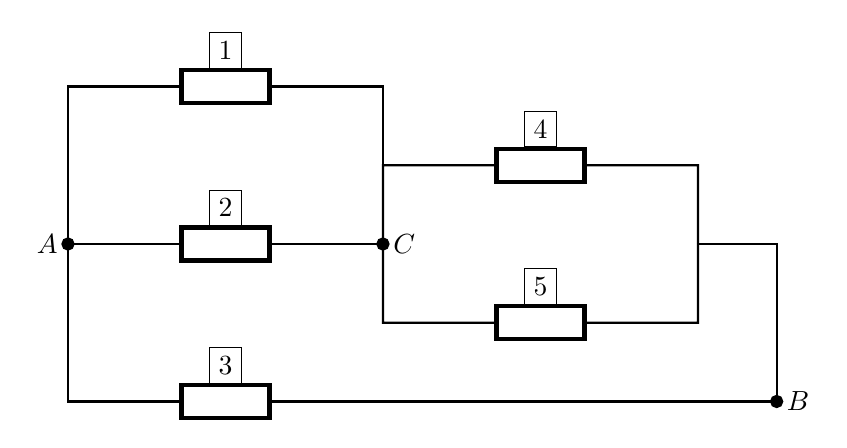
\begin{tikzpicture}[transform shape, thick]
size(2cm);
\ctikzset{bipoles/thickness=2}
\ctikzset{label/align = smart}
\coordinate  (A) at (0,0);
\coordinate  (B) at (9,-2);
\coordinate  (C) at (4,0);
\coordinate  (D) at (8,0);

\draw[fill=black] (A) circle (2pt) node[left] {$A$};
\draw[fill=black] (B) circle (2pt) node[right] {$B$};
\draw[fill=black] (C) circle (2pt) node[right] {$C$};

\draw (A) to ($(A) + (0, 2)$) to  [R, l=$\boxed{1}$] ($(C) + (0, 2)$) to (C);
\draw (A) to  [R, l=$\boxed{2}$] (C);
\draw (A) to ($(A) + (0, -2)$) to  [R, l=$\boxed{3}$] ($(C) + (0, -2)$) to (B);

\draw (C) to ($(C) + (0, 1)$) to  [R, l=$\boxed{4}$] ($(D) + (0, 1)$) to (D);
\draw (C) to ($(C) + (0, -1)$) to  [R, l=$\boxed{5}$] ($(D) + (0, -1)$) to (D);

\draw (D) to ($(B) + (0,2)$) to (B);
\end{tikzpicture}
\end{center}
We can break up this circuit into simpler components:
\begin{center}
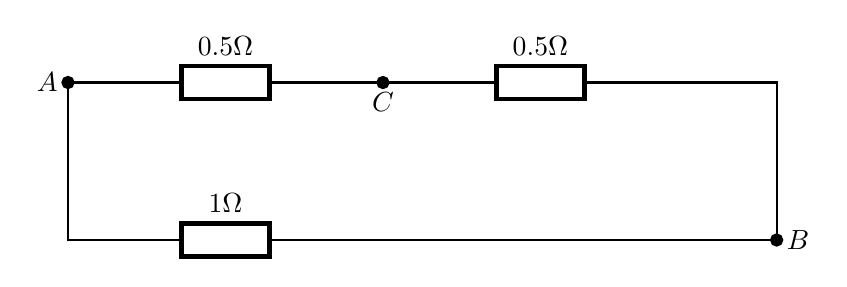
\begin{tikzpicture}[transform shape, thick]
size(2cm);
\ctikzset{bipoles/thickness=2}
\ctikzset{label/align = smart}
\coordinate  (A) at (0,0);
\coordinate  (B) at (9,-2);
\coordinate  (C) at (4,0);
\coordinate  (D) at (8,0);

\draw[fill=black] (A) circle (2pt) node[left] {$A$};
\draw[fill=black] (B) circle (2pt) node[right] {$B$};
\draw[fill=black] (C) circle (2pt) node[below] {$C$};

\draw (A) to  [R, l=$0.5\Omega$] (C);

\draw (C) to [R, l=$0.5\Omega$](D);
\draw (D) to ($(B) + (0,2)$) to (B);

\draw (A) to ($(A) + (0, -2)$) to  [R, l=$1\Omega$] ($(C) + (0, -2)$) to (B);
\end{tikzpicture}
\end{center}
and the equivalent resistance is:
$$R=\frac{(0.5+0.5)(1)}{1+(0.5+0.5)}=0.5\, \Omega$$
\end{solution}
\begin{solution}{easy}
The hint gives away the key to this problem. Due to symmetry, there is no current through the bridge resistor, hence it can be removed. Thus, this is the same as two 5 ohm resistors in parallel, so that gives us$$R_{eff} = \dfrac{1}{1/5+1/5} = \boxed{2.5 \, \Omega}.$$
\end{solution}
\begin{solution}{normal}
We use idea 6 and transform the circuit into two pairs of parallel resistors, with the pairs in series. The current $I$ that passes through the entire circuit is given by:
$$3 = I\left(\frac{(2)(2)}{2+2} + \frac{(3)(2)}{2+3}\right) \implies I = \frac{15}{11} \text{ A}$$As the current passes through the first pair of parallel resistors, the current is split half and half (since the two resistors are both $2\, \Omega$, such that a current of $i_1=\frac{15}{22} \text{ A}$ passes through the top left resistor.

As the current passes through the second pair of parallel resistors, the current is split in a ratio of $2:3$, so a current of $i_2=\frac{15}{11}\cdot \frac{2}{5} = \frac{6}{11}\text{ A}$ passes through the top right resistor.

The difference between these two currents is what passes through the bridge, which is:
$$I = \Delta i = \boxed{\frac{3}{22} \text{ A}}.$$
\tcbline
We can also approach this in a traditional way. We set up equations using Kirchoff's laws. Denote $I_1$ as the current through the bottom branch, $I_2$ as the current through the top branch and $I$ as the current through the ammeter. Then we can write out three loop equations which contain the voltage source:
\begin{align*}
2I_2+2(I+I_2) &= 3 & \text{(bottom loop)}\\
2I_2+3(I_2-I) &= 3 & \text{(top loop)}\\
2I_2 + 2(I+I_2) &= 3 & \text{(zig zag from top left)}
\end{align*}Here, we have let the current $I$ flow downwards in the bridge as the lower branch has a smaller resistance. Note that even if we had selected the wrong direction, our answer would be negative, so it can still be interpreted correctly. After solving this system of three equations, we find that $\boxed{I = \dfrac{3}{22}\,\mathrm{A}}$.
\end{solution}
\begin{solution}{normal}
The current through $V_1$ is $I_1$, so the resistance of the voltmeter is $R_v = \dfrac{V_1}{I_1} = 0.5 \, \mathrm{M\Omega}$. Thus the current through $V_2$ is $I_2 = V_2/R_v = 4\, \mathrm{\mu A}$. By Kirchoff's current junction rule, the current through the ammeter on the right is $I = I_1 - I_2 = \boxed{196 \, \mathrm{\mu A}}$.

The ammeter on the right has a large internal resistance of $R_A = \frac{V_2}{I}=10.2 \text{ k}\Omega$. If it was used to read the current, then the percent error would be $2\%$.
\end{solution}
\begin{solution}{hard}
First, note that all voltometers are identical while the ammeters are not. Since the voltometers, are identitcal, it would be wise to see the internal resistance that they have as it will most likely help to solve the problem. We are given the reading of the first ammeter to be $I_1 = 2.9\;\mathrm{mA}$ and the reading of the second ammeter to be $I_2 = 2.6\;\mathrm{mA}$. Therefore, the current drop is $\Delta I = 0.3\;\mathrm{mA}$. By fact 3 (Ohm's Law), we write:
\[r = V/\Delta I \implies r = 3\times 10^4\;\mathrm{\Omega}.\]Note that there is an extra factor of $10^{2}\;\mathrm{\Omega}$ since the current is measured in milliamperes. Now, by idea 8, we know that it is sometimes convenient to consider the Kirchoff’s current law for a whole region and not just for a single circuit node: the sum of currents entering the region equals to the sum of outgoing currents. In this case, we will consider the region marked by the circle below:

\begin{center}
    \includegraphics[width=0.6\linewidth]{Figures/7_sol.jpg}
\end{center}

The total voltage of the region will then be given by
\[V_{\text{region}} = \sum_{i = 2}^{15} V_i = \sum_{i = 2}^{15} r (I_i - I_{i  +1}) = r\sum_{i = 2}^{15} (I_i - I_{i  +1})\]where $i = 2, 3, \dots, 15$ represents a node in the circuit. The total voltage will then be given as
\begin{align*}
V_{\text{region}} &= r\sum_{i = 2}^{15} (I_i - I_{i  +1})\\
&= r(I_2-I_3) + \dots + r(I_{14}-I_{15}) + rI_{15}  \\
&= rI_2 \\
& = \boxed{78\;\mathrm{V}}.
\end{align*}
\end{solution}
\begin{solution}{normal}
First, note that by idea 9, this circuit can be turned into a $\Delta$ transform by merging the end nodes on both sides of the resistors as shown below 
\begin{center}
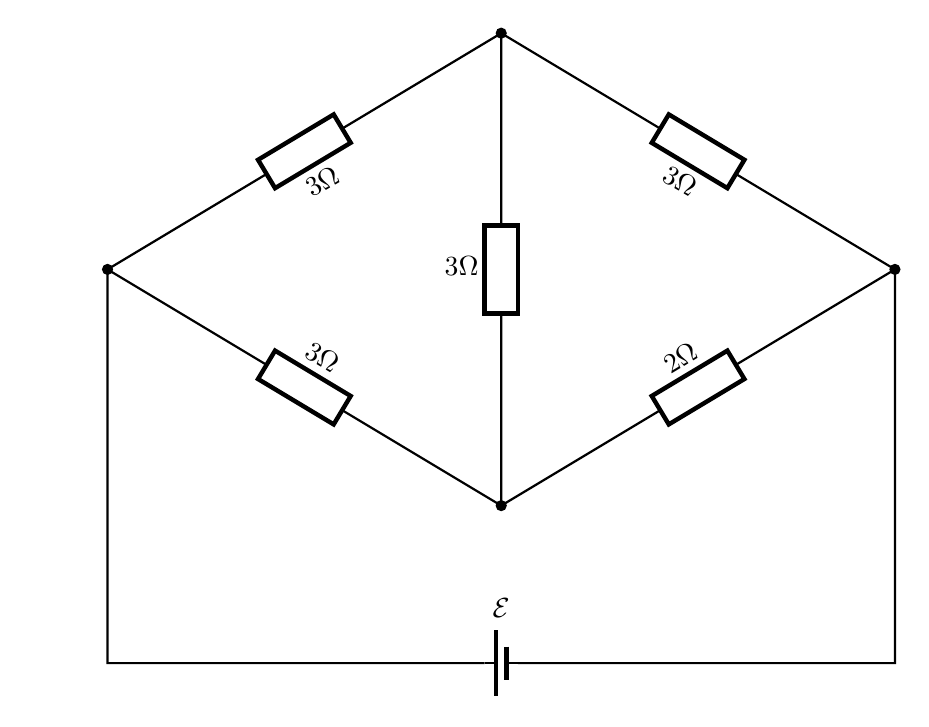
\begin{tikzpicture}[transform shape, thick]
size(2cm);
\ctikzset{bipoles/thickness=2}
\ctikzset{label/align = smart}
\draw (1, 4) -- (1, -1) to [battery1, l=$\mathcal{E}$] (11, -1) -- (11, 4);
\draw (1, 4) to [R, l=$3\Omega$] (6, 1) to [R, l=$3\Omega$] (6, 7) to [R, l=$3\Omega$] (1, 4);
\draw (6, 1) to [R, l=$2\Omega$] (11, 4);
\draw (11, 4) to [R, l=$3\Omega$] (6, 7);
\draw (6, 7) to [open, *-] (0, 0);
\draw (1, 4) to [open, *-] (0, 0);
\draw (6, 1) to [open, *-] (0, 0);
\draw (11, 4) to [open, *-] (0, 0);
\end{tikzpicture} 
\end{center}
We now apply a $\Delta$-to-$y$ transform on the lefthand $\Delta$ circuit. The resistances will change to 
\[R_A = \frac{R_{AB}R_{AC}}{R_{AB} + R_{AC} + R_{BC}} = \frac{9}{9}\Omega = 1\Omega.\]
Similarly, repeating this procedure for other indices, we see that our $y$ transform is simply just a $y$ transform with resistors of $1\Omega$ resistance. This can be represented as 
\begin{center}
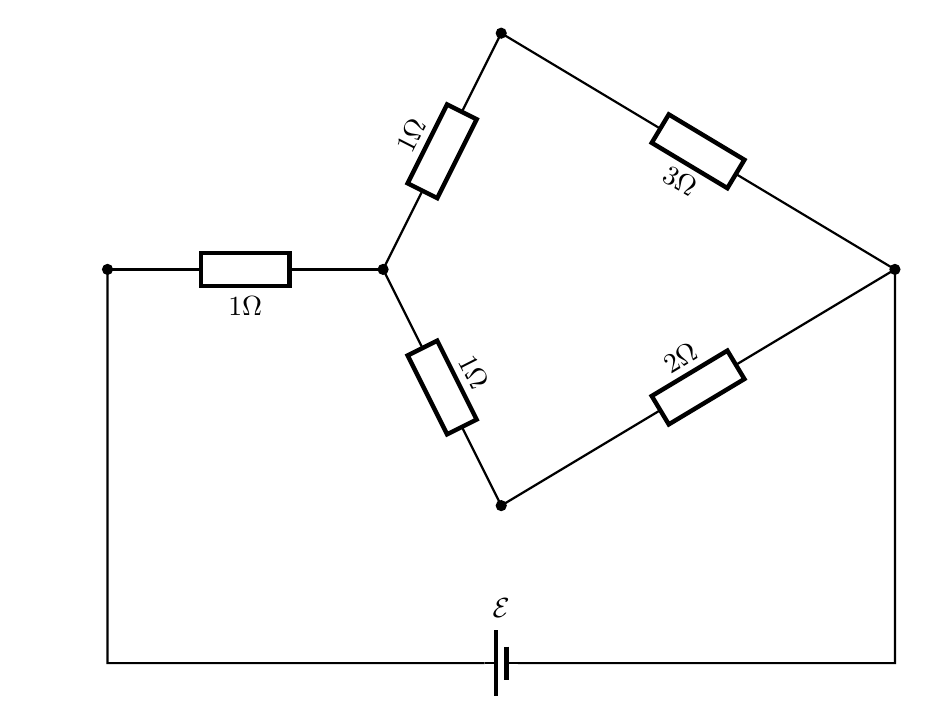
\begin{tikzpicture}[transform shape, thick]
size(2cm);
\ctikzset{bipoles/thickness=2}
\ctikzset{label/align = smart}
\draw (1, 4) -- (1, -1) to [battery1, l=$\mathcal{E}$] (11, -1) -- (11, 4);
\draw (6, 1) to [R, l=$2\Omega$] (11, 4);
\draw (11, 4) to [R, l=$3\Omega$] (6, 7);
\draw (4.5, 4) to [open, *-] (0, 0);
\draw (4.5, 4) to [R, l=$1\Omega$] (1, 4);
\draw (4.5, 4) to [R, l=$1\Omega$] (6, 1);
\draw (4.5, 4) to [R, l=$1\Omega$] (6, 7);
\draw (6, 7) to [open, *-] (0, 0);
\draw (1, 4) to [open, *-] (0, 0);
\draw (6, 1) to [open, *-] (0, 0);
\draw (11, 4) to [open, *-] (0, 0);
\end{tikzpicture} 
\end{center}
This circuit can be thought of as a connection between a resistor and two parallel resistors created by the top and bottom resistors added in series. In other words,
\begin{center}
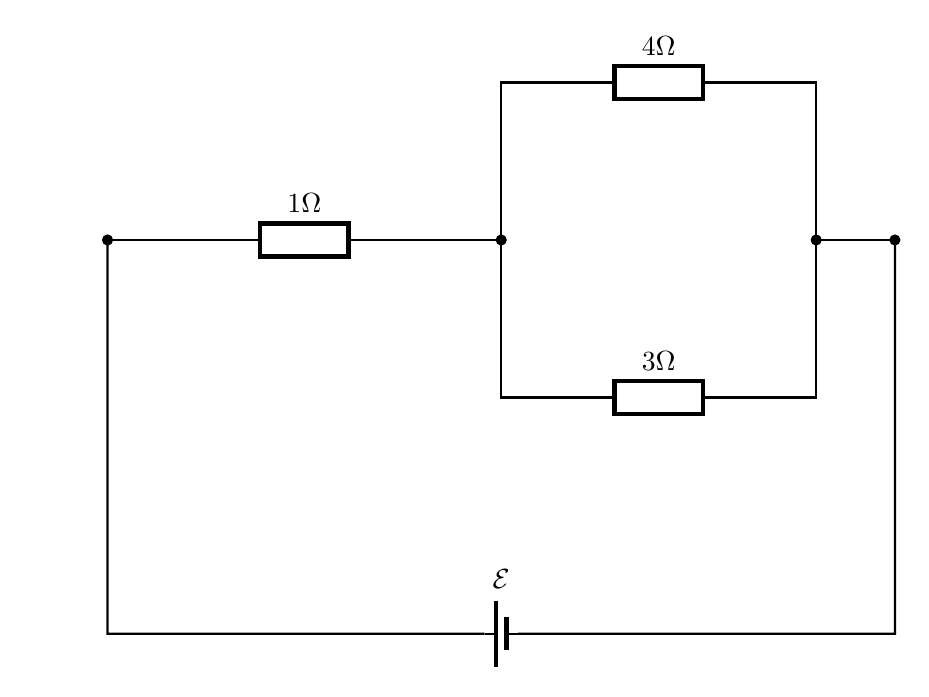
\begin{tikzpicture}[transform shape, thick]
size(2cm);
\ctikzset{bipoles/thickness=2}
\ctikzset{label/align = smart}
\draw (1, 4) -- (1, -1) to [battery1, l=$\mathcal{E}$] (11, -1) -- (11, 4);
\draw (1, 4) to [open, *-] (0, 0);
\draw (11, 4) to [open, *-] (0, 0);
\draw (1, 4) to [R, l=$1\Omega$] (6, 4);
\draw (6, 4) -- (6, 6) to [R, l=$4\Omega$] (10, 6) -- (10, 4) -- (11, 4);
\draw (6, 4) to [open, *-] (0, 0);
\draw (10, 4) to [open, *-] (0, 0);
\draw (6, 4) -- (6, 2) to [R, l=$3\Omega$] (10, 2) -- (10, 4);
\end{tikzpicture} 
\end{center}
By idea 1, 
\[\frac{1}{R_{\text{par}}} = \sum_i \frac{1}{R_i}\implies R_{\text{par}} = \frac{12}{7}\Omega.\]
Adding this to the $1\Omega$ resistor in series, we find that 
\[R_{\text{series}} = \sum_i R_i = \frac{19}{7}\Omega.\]
Our final circuit simply looks like 
\begin{center}
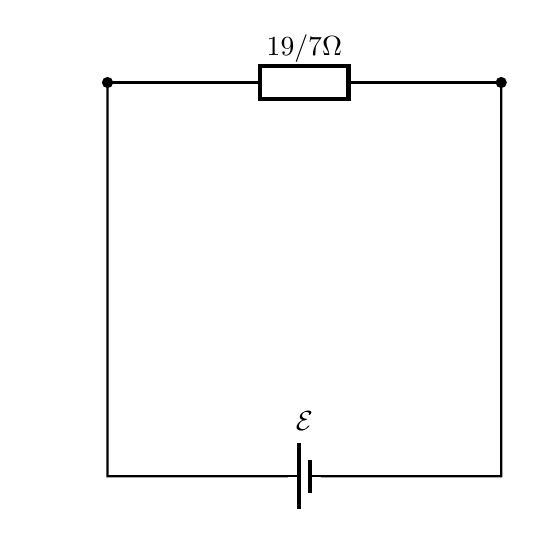
\begin{tikzpicture}[transform shape, scale=1.0,thick]
size(2cm);
\ctikzset{bipoles/thickness=2}
\ctikzset{label/align = smart}
\draw (1, 4) -- (1, -1) to [battery1, l=$\mathcal{E}$] (6, -1) -- (6, 4);
\draw (1, 4) to [open, *-] (0, 0);
\draw (6, 4) to [open, *-] (0, 0);
\draw (1, 4) to [R, l=$19/7\Omega$] (6, 4);
\end{tikzpicture} 
\end{center}
The current flowing through will then be given by fact 1 (Ohm's law):
\[R = V/I\implies I = V/R = \frac{3}{19/7} = \frac{21}{19}\;\mathrm{A}.\]
\end{solution}
\begin{solution}{normal}
The handout describes how to solve this problem. To summarize, the load is the $3\;\mathrm{V}$ battery, so we can remove it and then short the voltage source to calculate the Thevenin resistance. We then get $1 \Omega$ resistors in parallel connected in series to $2 \Omega$ resistors in parallel. The effective resistance is then $R_{\text{eq}} = 1.5 \Omega$. Now, the current through the $3\;\mathrm{V}$ battery can be calculated to be $\frac{3\;\mathrm{V}}{1.5 \Omega} = \boxed{2\;\mathrm{A}}.$
\tcbline
Alternatively, we can apply idea 12. We can set up the following systems of equations:
\begin{align*}
3 &= 1\left(I-I_1\right) + 2\left(I-I_1+I_2\right) & \text{(top loop)} \\ 
3 &= 1\left(I_1\right) + 2\left(I_1-I_2\right) & \text{(bottom loop)} \\ 
3 + 4 &= 1\left(I_1\right) +  2\left(I-I_1+I_2\right) & \text{(zig zag from bottom left)}
\end{align*}
Here, $I$ is the current through the battery of interest, $I_1$ is the current through the $1\Omega$ resistor in the bottom branch, and $I_2$ is the current through the bridge. Solving this system of equations gives $I=2\text{ A}$. The reason why the voltage of the bridge battery does not matter is that this value of $I$ allows the first two equations to be exactly identical.
\end{solution}
\begin{solution}{normal}
By idea $10$, any circuit which consists of only resistors and batteries and has two ports $A$ and $B$ is equivalent to a series connection of a battery and a resistance. In other words, we consider the Thevenin equivalent of the circuit. The equivalent internal resistance can be found easily replacing the battery by a wire and using series and parallel connections.
$$R_{\text{eq}} = \frac{R_2\times (R_1+r)}{R_2 + (R_1+r)}$$The equivalent emf $\mathcal{E}_{\text{eq}}$ is the potential drop across $R_2$. The net resistance about the battery is $R_2 + (R_1+r)$, so the current through the battery is by idea 10,
\[ I = \mathcal{E}/r\implies I = \frac{\mathcal{E}}{R_1+R_2+r}.\]The potential drop about $R_2$ is then
\[V = IR_2 = \mathcal{E}\frac{R_2}{R_1+R_2+r}.\]This means that entire circuit in the figure can be substituted with an equivalent battery with
$$\mathcal{E}_{\text{eq}} = \mathcal{E}\frac{R_2}{R_1+R_2+r}.$$By fact $7$ the maximal power that can be dissipated is given as $P_{\text{max}} = \mathcal{E}^2/4r$. This means that
\begin{align*}
P_{\text{max}} = \frac{\mathcal{E}_{\text{eq}}^2}{4R_{\text{eq}}} &= \frac{1}{4}\mathcal{E}^2 \left(\frac{R_2}{R_1+R_2+r}\right)^2 \cdot \frac{R_2 + (R_1+r)}{R_2\times (R_1+r)} \\
&= \frac{1}{4}\frac{R_2}{(r + R_1 + R_2)(R_1 + r)}\mathcal{E}^2
\end{align*}
\end{solution}
\begin{solution}{normal}
We apply idea 11 and we treat the batteries as $n$ current sources providing a current of $I_i = \dfrac{\mathcal{E}_i}{r_i}$. When determining an equivalent circuit, all the current sources add up to a total current of:
$$I_\text{total} = \sum_{i=1}^n \frac{\mathcal{E}_i}{r_i}$$and applying idea 11 again, this is equivalent to an effective voltage source of $\mathcal{E}_\text{eff} = I_\text{total}R_\text{eff}$ with the effective resistance being:
$$R_\text{eff} = \left(\sum_{i=1}^nr_i^{-1}\right)^{-1}$$since we are adding resistors in parallel. Putting everything together gives:
$$\mathcal{E}_\text{eff} = \left(\sum_{i=1}^nr_i^{-1}\right)^{-1}\sum_{i=1}^n \frac{\mathcal{E}_i}{r_i}$$
\end{solution}
\begin{solution}{normal}
We make use of idea 12 and start by short-circuiting $\mathcal{E}_2$. This leads to the following equivalent circuit:
\begin{center}
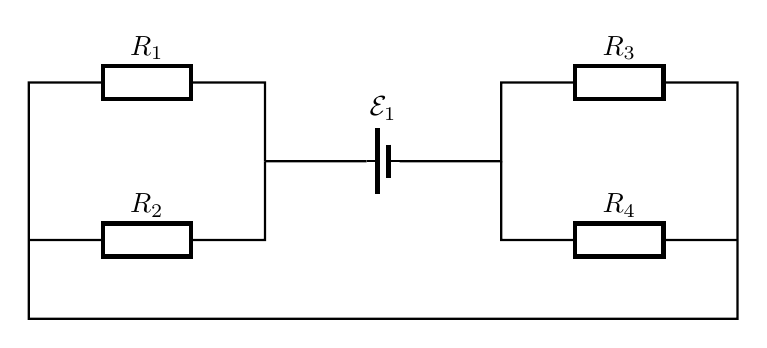
\begin{tikzpicture}[transform shape, thick]
\ctikzset{bipoles/thickness=2}
\ctikzset{label/align = smart}
\coordinate  (A) at (0,0);
\coordinate  (B) at (3,0);
\coordinate  (C) at (6,0);
\coordinate  (D) at (9,0);

\draw (B) to [battery1, l=$\mathcal{E}_1$] (C) to ($(C) + (0,1)$) to [R, l=$R_3$] ($(D) + (0,1)$) to ($(D) + (0,-2)$) to ($(A) + (0,-2)$) to ($(A) + (0,1)$) to [R, l=$R_1$] ($(B) + (0,1)$) to (B);

\draw ($(A) + (0,-1)$) to [R, l=$R_2$] ($(B) + (0,-1)$) to (B);
\draw (C) to ($(C) + (0,-1)$) to [R, l=$R_4$] ($(D) + (0,-1)$);
\end{tikzpicture}
\end{center}
Since all resistors have a resistance of $R$, this leads to the following currents in each resistor (going back to the original diagram):
\begin{align*}
    R_1 &\rightarrow \frac{\mathcal{E}}{2R} \, \text{(downwards)} \\ 
    R_2 &\rightarrow \frac{\mathcal{E}}{2R} \, \text{(rightwards)} \\ 
    R_3 &\rightarrow \frac{\mathcal{E}}{2R} \, \text{(downwards)} \\
    R_4 &\rightarrow \frac{\mathcal{E}}{2R} \, \text{(leftwards)}
\end{align*}
and similarly if we short $\mathcal{E}_1$, we get the following currents:
\begin{align*}
    R_1 &\rightarrow \frac{\mathcal{E}}{2R} \, \text{(downwards)} \\ 
    R_2 &\rightarrow \frac{\mathcal{E}}{2R} \, \text{(leftwards)} \\ 
    R_3 &\rightarrow \frac{\mathcal{E}}{2R} \, \text{(downwards)} \\
    R_4 &\rightarrow \frac{\mathcal{E}}{2R} \, \text{(rightwards)}
\end{align*}
By considering the superposition of these currents, we get after adding them together:
\begin{align*}
    R_1 &\rightarrow \frac{\mathcal{E}}{R} \, \text{(downwards)} \\ 
    R_2 &\rightarrow 0 \\ 
    R_3 &\rightarrow \frac{\mathcal{E}}{R} \, \text{(downwards)} \\
    R_4 &\rightarrow 0
\end{align*}
\tcbline
Alternatively we can solve this problem via symmetry. Note that there is reflection symmetry across the vertical line. This means that the current does not have a preferred direction of going either right or left, so that the current in $R_2$ and $R_4$ will be zero. As a result, we can simply replace these two resistors with an open gap, which results in the other four circuit elements in series:
$$    I = \frac{2\mathcal{E}}{2R} = \frac{\mathcal{E}}{R}
$$
which travels in a ``zigzag'' pattern.
\end{solution}
\begin{solution}{normal}
Provided in the handout.
\end{solution}
\input{14}
\begin{solution}{normal}
Note that in the dual circuit drawn, all resistors have a resistance one quarter of that of a corresponding resistor in the original circuit.
\begin{center}
    \includegraphics[width=0.6\linewidth]{Figures/pr15_sol.PNG}
\end{center}
For example, we have $a=d=1\,\Omega$, $c=b=0.25\,\Omega$, and $e=0.5\,\Omega$. These are obtained by letting the conductance of the original resistor elements the circuit passes through be the resistance of the dual resistors. Here, $a$ and $d$ correspond to one fourth of the $4\,\Omega$ resistors, $b$ and $c$ correspond to one fourth of the $1\,\Omega$ resistors and $e$ corresponds to one fourth of the $2\,\Omega resistors$. Therefore, we can say that:
$$R^* = \frac{R}{4}$$
where $R^*$ is the effective resistance of the dual circuit and $R$ is the effective resistance of the original circuit. However, from the stream function method, we must also have:
$$R^* = \frac{1}{R}$$
so we get:
$$\frac{R}{4}=\frac{1}{R} \implies \boxed{R=2\,\Omega}$$
\end{solution}
\begin{solution}{normal}
According to idea 18,  we “cut off” the first period of the infinite chain ; the remaining part is equivalent to the original circuit of (yet unknown) resistance $R$. 
\begin{center}
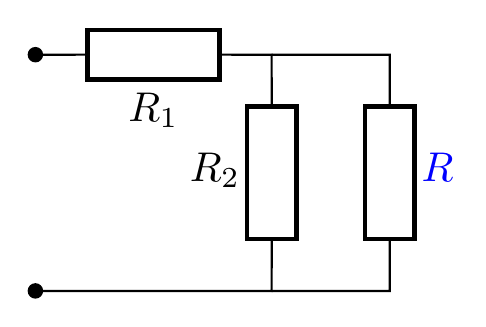
\begin{tikzpicture}[transform shape, scale=1.5, thick]
\ctikzset{label/align = smart}
\draw (0, 0) to [open, *-] (0, 1);
\draw (0, 2) to [open, *-] (0, 0);
\draw (0, 0) -- (2, 0) to [R, l=$R_2$] (2, 2) to [R, l=$R_1$] (0, 2);
\draw (2, 2) -- (3, 2) to [R, l=$R$, blue] (3, 0) -- (2, 0);
\end{tikzpicture}
\end{center}
Because of that, we can write equality
\[R = R_1 + \frac{R R_2}{R + R_2}\]
which upon cross multiplying, gives us the equation 
\[R^2 - RR_1 - R_1 R = 0\implies R = \frac{R_1}{2}\left(1 + \sqrt{1 + \frac{4R_2}{R_1}}\right)\]
by the quadratic equation.
\end{solution}
\begin{solution}{normal}
According to idea 18,  we “cut off” the first period of the infinite chain ; the remaining part is equivalent to the original circuit of (yet unknown) resistance $R'$ and an electromotive force of $\mathcal{E}'$. 
\begin{center}
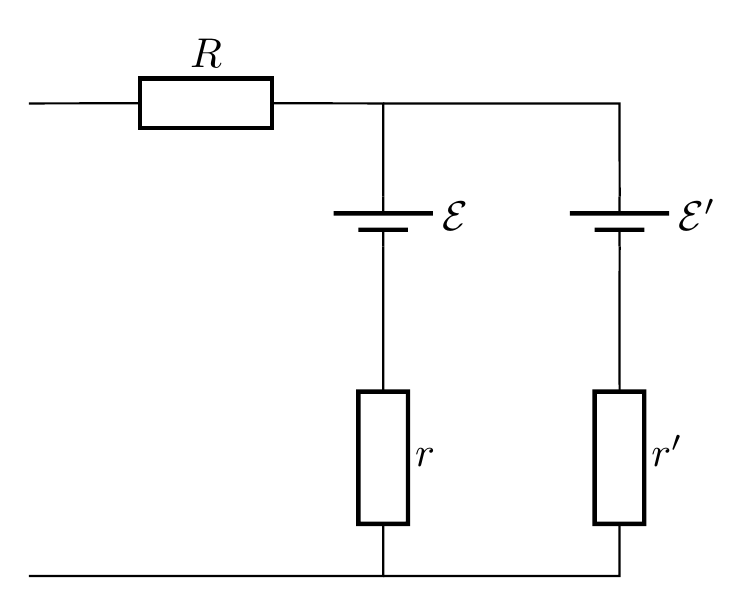
\begin{tikzpicture}[transform shape, scale=1.5, thick]
\ctikzset{label/align = smart}
\coordinate (A) at (0,0);
\coordinate (B) at (3,0);
\coordinate (C) at ($(B) + (2,0)$);
\coordinate (D) at ($(C) + (0,4)$);
\coordinate (E) at ($(B) + (0,4)$);
\coordinate (F) at (0,4);
\draw (F) to [R, l=$R$] (E) to [battery1, l=$\mathcal{E}$] ($(E)!0.5!(B)$) to [R, l=$r$] (B) to (A);
\draw (E) to (D) to [battery1, l=$\mathcal{E}'$] ($(D)!0.5!(C)$) to [R, l=$r'$] (C) to (B);
\end{tikzpicture}
\end{center}
We apply Thevenin's theorem to solve this. First, we remove all voltage and current sources and write the effective resistance $r'$ to be:
\begin{align*}
    r' &= R + \frac{rr'}{r+r'} \\ 
    0 &= {r'}^2-Rr'-Rr \\ 
    r' &= \frac{R}{2} \left(1+\sqrt{1-\frac{4r}{R}}\right)
\end{align*}
We can also calculate the effective Thevenin voltage by letting $\mathcal{E}'$ be the voltage across the gap. No current will be flowing through $R$, so this will be the current that flows through the $\mathcal{E}$ battery. We can determine the current to be (assuming it moves clockwise):
$$
    I_\text{th} = \frac{\mathcal{E}-\mathcal{E}'}{r+r'}
$$
and the effective voltage to be:
$$
\mathcal{E}' = \mathcal{E} - I_\text{th}r \implies \mathcal{E}' = \mathcal{E}
$$
\end{solution}
\begin{solution}{easy}
We notice that there are certain nodes on the cube (due to symmetry), that have the same potential as illustrated below:
\newcommand{\Depth}{4}
\newcommand{\Height}{4}
\newcommand{\Width}{4}
\begin{center}
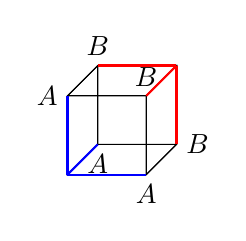
\begin{tikzpicture}
\coordinate (O) at (0,0,0);
\coordinate (A) at (0,\Width,0);
\coordinate (B) at (0,\Width,\Height);
\coordinate (C) at (0,0,\Height);
\coordinate (D) at (\Depth,0,0);
\coordinate (E) at (\Depth,\Width,0);
\coordinate (F) at (\Depth,\Width,\Height);
\coordinate (G) at (\Depth,0,\Height);

% \draw[fill=black] (C) node[left] {$C$};
\draw[fill=black] (O) node[below] {$A$};
\draw[fill=black] (G) node[below] {$A$};
\draw[fill=black] (B) node[left] {$A$};

\draw[fill=black] (F) node[above] {$B$};
\draw[fill=black] (A) node[above] {$B$};
\draw[fill=black] (D) node[right] {$B$};
% \draw[fill=black] (E) node[right] {$B$};

\draw[black] (O) -- (C) -- (G) -- (D) -- cycle;
\draw[black] (O) -- (A) -- (E) -- (D) -- cycle;
\draw[black] (O) -- (A) -- (B) -- (C) -- cycle;
\draw[black] (D) -- (E) -- (F) -- (G) -- cycle;
\draw[black] (C) -- (B) -- (F) -- (G) -- cycle;
\draw[black] (A) -- (B) -- (F) -- (E) -- cycle;

\draw[blue, thick] (C) -- (O);
\draw[blue, thick] (C) -- (G);
\draw[blue, thick] (C) -- (B);

\draw[red, thick] (E) -- (A);
\draw[red, thick] (E) -- (D);
\draw[red, thick] (E) -- (F);
\end{tikzpicture}
\end{center}
We can shortwire the connections between the ends of all resistors with the same color (e.g. identically labeled nodes have the same potential) to transform it to the following circuit:
\end{solution}
\input{19}
\begin{solution}{hard}
Provided in handout. 
\end{solution}
\begin{solution}{hard}
\textbf{Method 1.} Let us consider what happens when we drive a current $I$ through node $A$ such that there will be a current $I/20$ through every vertex including $A$. By Kirchhoff's Laws and by the symmetry of the dodecahedron, we have the current that is going in $A$ to be
\[I_A = \frac{I-I/20}{3} = \frac{19}{60}I.\]Now, we attempt to superpose this current such that the $I/20$ vanishes from each vertex. The only way to do so is to feed the same current $I_A$ through the adjacent vertex $B$, however with a negative current. The $\pm I/20$ current through each vertex cancels out except the edge that connects $A$ and $B$. This edge will contain a current
\[I’ = I_A - I_B = \frac{19}{30}I\]By Ohm’s Law, this implies the resistance is $\boxed{\frac{19}{30}R}$.
\tcbline
\textbf{Method 2.} There are $E=30$ resistors, each resistor with an effective resistance $r$. The number of vertices is $V=20$. By Foster's Theorem:
$$Er=(V-1)R \implies r = \frac{V-1}{E}R = \frac{19}{30}R$$
\end{solution}
\begin{solution}{hard}
We use the idea of "negative resistance". In this case, the edge connecting vertices $\text{A}$ and $\text{B}$ is cut off. We can represent the missing wire as a parallel connection of $R$ and $-R$. This is because idea 22 tells us that a resistor and a negative resistor in parallel corresponds to infinite resistance which is what $\text{AB}$ essentially is since no current can flow through. From problem 21, we note that
\[R = \frac{19}{30}R\]and since we have a $R$ and $-R$ resistor in parallel (as shown below)
\begin{center}
\begin{asy}
size(6cm);
draw((0,0) -- (0.5, 0));
dot((0.5, 0));
draw((0.5, 0) -- (0.5, 0.25));
draw((0.5, 0) -- (0.5, -0.25));
draw((0.5, 0.25) -- (1.5, 0.25), purple + blue);
label("$R$", (1, 0.25), N);
draw((0.5, -0.25) -- (1.5, -0.25), purple + red);
draw((1.5, -0.25) -- (1.5, 0.25));
dot((1.5, 0));
draw((1.5, 0) -- (2, 0));
label("$-R$", (1, -0.25), S);
label("A", (0.5, 0), NW);
label("B", (1.5, 0), NE);
\end{asy}
\end{center}
We can reduce the equivalent resistance by idea 1:
\[\frac{1}{R_{\text{eq}}} = \sum_{i} \frac{1}{R_{i}} = \frac{1}{R} + \frac{1}{-R}\implies R_{\text{eq}} = \frac{(\frac{19}{30}R)(-R)}{\frac{19}{30}R - R} = \frac{19}{11}R.\]
\end{solution}
\begin{solution}{normal}
We first find when the voltage on the left component reaches 1. If there's a voltage $V$ on the circuit, Since the current will split evenly, the left component will have a voltage drop of $2V/3$. So the first transition occurs at $1.5 \,V$ so at 1.5 s. At this point the voltage drop across the left component is 1 V, and since it has a resistance of 1 ohm, the current is 1 A. After the change, there is still a voltage drop of 1 V, and a resistance of 2 ohms, but now $4/5$ of the voltage drop occurs at this component since it has double the resistance and current compared to the other components. Thus there is a voltage drop of 0.6 V. We continue this calculation for every single transition.

The next transition occurs when $V/5 = 1\, V$ since 1/5 of the voltage drop occurs on the right components. This is at 5 V or 5 s. The current is then 2 A as there is 4 V across the 2 ohm component. Then the resistors become 2 ohms, and then we calculate that he current is $5\dfrac{2}{3}\dfrac{1}{2} = 5/3\, A$. Now this will go until the peak at 10 V, where there is a current of 10/3 A.

The next transition occurs at 3 V since 1/3 of the voltage drop occurs on the right components, so $V/3 = 1$ is at 3 V. Here the current is 1 A and then 1.2 A. The final transition occurs at 5/4 V since $4/5$ of the voltage drop occurs on the left component. Here the current is 0.5 A and then 5/6 A.
\end{solution}
\begin{solution}{normal}
Let the diode have a potential difference (p.d.) of $V$. By idea 24, it is quite apparent that the p.d. across the reistor will be 
\[1.5 - V = I r.\]
Taking $i$ to be in mA which means $i = 1000 I$, we find that 
\[i (V) = 15 - 10 V.\]
We also have the equation of the current voltage graph $I(V)$, which allows to find the intersection between this line and the graph. 
\begin{center}
    \includegraphics[width=7cm]{49B62025-1343-4881-9854-3AF244D6DE23.jpeg}
\end{center}
\end{solution}
\input{25}
\input{26}
\input{27}
\input{28}
\input{29}
\input{30}
\input{31}
\input{32}
\input{33}
\input{34}
\input{35}
\input{36}
\input{37}
\input{38}
\input{39}
\input{40}
\input{41}
\input{42}
\input{43}
\input{44}
\input{45}
\input{46}
\input{47}
\input{48}
\input{49}
\input{50}
\begin{solution}{normal}
According to idea 18,  we “cut off” the first period of the infinite chain ; the remaining part is equivalent to the original circuit of (yet unknown) resistance $2R_{\infty}$. 
\begin{center}
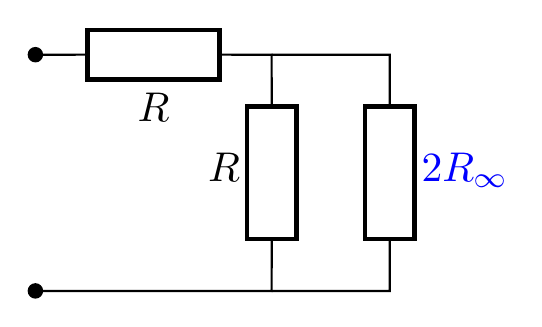
\begin{tikzpicture}[transform shape, scale=1.5, thick]
\ctikzset{label/align = smart}
\draw (0, 0) to [open, *-] (0, 1);
\draw (0, 2) to [open, *-] (0, 0);
\draw (0, 0) -- (2, 0) to [R, l=$R$] (2, 2) to [R, l=$R$] (0, 2);
\draw (2, 2) -- (3, 2) to [R, l=$2R_{\infty}$, blue] (3, 0) -- (2, 0);
\end{tikzpicture}
\end{center}
Because of that, we can write equality
\[R_{\infty} = R + \frac{2RR_{\infty}}{2R_{\infty} + R}\]
which upon cross multiplying, gives us the equation 
\[2R_{\infty}^2 - 3RR_{\infty} - R^2 = 0\implies R_{\infty} = \frac{1}{4}R(3 + \sqrt{17})\]
upon taking the positive root by the quadratic equation.
\end{solution}
\input{52}
\input{53}
\input{54}
\begin{solution}{hard}
Consider two nodes in the circuit indexed by $i$ and $j$. We can find an expression between the $i$-th and $j$-th node if they are connected. Let $\varphi_{k}^{(i\to j)}$ represent the potential of the $k$-th node in the circuit where $2\leq k \leq n$ with respect to current $I$ that is driven into the $i$-th node and driven out of the $j$-th node. The resistance $R_{ij}$ between these two nodes (if they are connected) can then be expressed as
\[R_{ij} = \frac{\left(\varphi_{i}^{(i\to j)} - \varphi_{j}^{(i \to j)}\right)}{I}.\]
The resistance between all adjacent nodes will be summed up to find the total resistance. This means that we wish to find a sum for all $i, j$-th nodes in the system. To do this, our current expression of finding the resistance is not satisfactory as we don't have terms for the resistance of the resistors. If we multiply both sides with the electrical conductance $\sigma_{ij} = 1/R$, we find that (notice how we were also able to get rid of the potentials $\varphi$ with this!)
\[
\frac{R_{ij}}{R} = \frac{\left(\varphi_{i}^{(i\to j)} - \varphi_{j}^{(i \to j)}\right)}{IR} \implies R_{ij} = \frac{\left(I_{i}^{(i\to j)} - I_{j}^{(i \to j)}\right)}{I}R.
\]
Now, the setup of current $I$ going into the $i$-th node and coming out of the $j$-th node will be the sum of a superposition of two different setups:
\begin{itemize}
    \item From the other $n - 1$ points, we will take a current of $I/n$ into the $j$-th node and we will put a current of $(1 - I/n)$ into the $i$-th node. 
    \item We will take out a current of $(1 - I/n)$ out of the $j$-th node and then put a current of $I/n$ (it is $I/n$ because $(1 - I/n) = (n - 1)I/n$ which means when it goes into the other $n - 1$ nodes, only a current of $I/n$ will be needed) into the other $n -1$ points
\end{itemize}
This means that in our expression of resistance, each node pair will be counted twice. So, noting that $I_k^{(i \to j)} = I_k^{(i)} - I_k^{(j)}$ and the previous fact allows us to take the sum $\sum_{i, j} R_{ij} = \sum_{i}\sum_{j} R_{ij}$. Hence, 
\begin{align*}
    2\sum_{ij} R_{ij} &= \left(\sum_{i}\sum_{j} \frac{\left(I_{i}^{(i)} - I_{i}^{(j)} - I_{j}^{(i)} + I_{j}^{(j)}\right)}{I}\right)R \\
    &= \left(\sum_{i} \frac{I_{i}^{(i)} - I_{i}^{(j)}}{I} + \sum_{j} \frac{I_{j}^{(i)} + I_{j}^{(j)}}{I}\right)R.
\end{align*}
Both sums are essentially part of the superposition argument written above. If a current of $(n - 1)I/n$ enters each point from $n$ currents entering $n$ points, then the sum essentially equals $(n - 1)$. The same argument can be said for the second sum and we yield that 
\[\sum_{ij} R_{ij} = (n - 1)R.\]
$\square$
\end{solution}

\newpage
\section{Circuits including Capacitors and Inductances}
\vspace{-5mm}

\input{56}
\input{57}
\input{58}
\input{59}
\input{60}
\input{61}
\input{62}
\input{63}
\input{64}
\input{65}
\input{66}
\input{67}
\begin{solution}{normal}
The magnetic flux on the coil changes rapidly from $\Phi_1 = +NBS$ to $\Phi_2 = -NBS$. Thus, the total change in flux is given to be $\delta \Phi_e = 2NBS$. As the coil moves in a fast motion, the change in current is too small to give any difference, so $\delta I \approx 0$. By idea 41, one can write that the charge passing through the wires is $q = (\delta \Phi_e + L\delta I)/R\implies q = 2NBS/R$.
\end{solution}
\input{69}
\input{70}
\input{71}
\input{72}
\input{73}
\begin{solution}{normal}

\end{solution}
\input{75}
\begin{solution}{normal}
\begin{enumerate}[label = (\alph*)]
\item Due to idea 38, inductors can be considered as a short circulating wire while the capacitator charge is almost constant. Because of that, there will be no current going through the capacitator and we can effectively remove them from the circuit. This also implies that there will be no current going through $R_1$, which then implies that the voltometer will show $R_2 = \boxed{\mathcal{E}}$.

\item After the switch is opened, there is immediately a current of $\mathcal{E}/R$ flowing through the inductors. This means that the current through $R_1$ and $R_2$ is $\mathcal{E}/R$ as well. Thus the voltage through $R_1$ will be $3R\frac{\mathcal{E}}{R}$ while the voltage through $R_2$ will be $R\frac{\mathcal{E}}{R}$. The voltometer will then read the difference as $-2\mathcal{E}$.

\item Using the hint, we apply energy conservation (notice that the circuit breaks down into two independent circuits, so that the power dissipation can be calculated separately for each of the circuits).

After opening both switches, the capacitator $C_1$ has no charge (since it is connected to $R_1$ which contains no current) and the capacitator $C_2$ has a charge $\mathcal{E}$. Since the voltometer has a large resistance, we can effectively disonnect it from the system. Also, note that $L_1$ and $L_2$ carry a current $\mathcal{E}/R_2$. This means that, as we said, the circuit breaks down into two independent circuits. 
\begin{itemize}
\item Circuit 1: $R_1L_1C_1$
\item Circuit 2: $R_2L_2C_2$
\end{itemize}
Remember that the energy of a capacitor is $E_c = \frac{1}{2}C\mathcal{E}^2$ while the energy through the inductor will be $E_{L} = \frac{1}{2}LI^2 = \frac{1}{2}L\frac{\mathcal{E}^2}{R^2}$. Note that the circuit can be split into two individual triangles of components $C_1, R_1, L_1$ and $R_2, C_2, L_2$. 

Thus, we can sum up the energies in each individual circuit. For circuit 1, the energy dissipated is simply $\frac{1}{2}L\frac{\mathcal{E}^2}{R^2}$ while in the second circuit, $\mathcal{E}^2 \left(\frac{C}{2} + \frac{L}{2R^2}\right)$. 
\end{enumerate}
\end{solution}
\input{77}
\input{78}
\input{79}
\input{80}
\input{81}
\begin{solution}{hard}
We neglect $L_d$ and $C_d$. By idea 31, assume the departure from the stationary state is very small, and a perturbation current $\widetilde{I}$ is described by a circuit obtained by substituting the diode with a resistance $R_{\text{diff}}$ and removing the electromotive force. To find stabilizing conditions, we can use idea 41 or write a DE with KVL. 
\\
\\
In the steady state, let the deviation of charge of the capacitor in a period be $\delta q$. By KVL in the smaller loop, $\delta I (R_{\text{diff}} + r) = \delta q/C$. By differentiating, we can see that $\delta \dot q = \delta \dot I (R_{\text{diff}} + r)C$. Both these currents combine or superimpose at the end nodes which means that the current through $R$ and $L$ is $\delta I + \delta \dot q$. We can now write KVL for the whole circuit as 
\[(\delta I + \delta \dot q) R + L \frac{\text{d}}{\text{d}t}\left( \delta I + \delta \dot q\right) + \delta I (R_{\text{diff}} + r) = 0.\]
Rearranging and substituting 
\begin{align*}\delta \ddot I(R_{\text{diff}} + r)LC + \delta \dot I\left(L +  (R_{\text{diff}} + r)RC\right) + \delta I(R_{\text{diff}} + r + R) &= 0 \\
\delta \ddot I + \delta \dot I \left(\frac{1}{(R_{\text{diff}} + r)C} + \frac{R}{L}\right) + \delta I \left(\frac{R_{\text{diff}} + r + R}{(R_{\text{diff}} + r)LC}\right) &= 0 
\end{align*}
Thus, we can write the differential equation in the form of $\delta \ddot I + \delta \dot I \xi + \delta I \eta = 0$. We can solve this differential equation by finding the characteristic equation using the general solution of:
\[\delta I = A \exp (\lambda_1 t) + B \exp (\lambda_2 t)\]
where $\lambda$ is the solution to the characteristic equation $\lambda^2 + \xi \lambda + \eta = 0$, when $\lambda_1 \neq \lambda_2$. It is apparent that the solutions to this characteristic equation follows the quadratic equation or 
\[\lambda_{1, 2} = -\frac{\xi}{2} \pm \sqrt{\frac{\xi^2}{4} - \eta}.\]
Depending on the value of the discriminant, the solution to this equation can be either real or complex. Generally, we can write that $\lambda_i = \gamma_i \pm i\omega_i$ such that $\omega_i = 0$ if $\lambda_i \in \mathbb R$. Thus, by superimposing both real and complex solutions, we have that 
\[\delta I = \sum_{i = 1}^{2} \delta I_{0i} e^{\gamma_i t} \left( \cos (\omega_i t) + i\sin (\omega_i t)\right).\]
From this, $\gamma < 0$ for the solution to be exponentially decaying to reach a steady state. This will stabilize the diode. Since $\gamma < 0$ and $\gamma = -\xi/2$, then $\xi > 0$. This means that 
\[\frac{1}{(R_{\text{diff}} + r)C} + \frac{R}{L} > 0\implies \frac{L}{C} < R |R_{\text{diff}}| + rR.\]
By applying the condition of $\eta > 0$, it is found that $R_{\text{diff}} + r + R > 0$. 
\\
\\
For very fast perturbations, the impedance of the inductance $L$ can be considered infinitely large, hence no current can enter the inductor $L$ and resistor $R$: this part of the circuit can be “cut off”. Similarly, for such fast processes, the impedance of the capacitor $C$ is negligibly small, so it can be short-circuited in the equivalent circuit. Now rewriting the circuit, we can once again procede in the same way as part (a) by writing Kirchoff's laws. This gives us a similar condition of $L_d < r|R_{\text{difff}}|C_d$. 
\\
\\
Refer to the tunnel diode problem from the 2020 NBPhO for a problem with a quite similar analysis. 
\end{solution}
\input{83}
\input{84}
\input{85}
\input{86}
\input{87}
\begin{solution}{normal}
First, disregard the capacitor and consider a current $I$ that flows through the toroidal ferromagnet. We can consider the ferromagnet to be made of two inductors (each consists of a half on each side). Because of this, there will be a mutual inductance $M$ present as well. It is known by fact 21 that $M$ cannot be greater than the geometric average of both inductors i.e. $M = \sqrt{L_1 L_2}$ is achieved for transformers when all the magnetic field lines created by the both coils have identical shapes. Let the inductance of one half be $L'$ such that by symmetry, the inductance of the other half is also $L^\prime$; therefore, $M = \sqrt{L^{\prime 2}} = L^{\prime}$. We find that the voltage induced on one half of the ferromagnet will follow $L^\prime \frac{\text{d}I}{\text{d}t} + M \frac{\text{d}I}{\text{d}t} = 2L^\prime \frac{\text{d}I}{\text{d}t}$. Thus, the total voltage induced will be two times this (as there are two halves) or $4L^\prime \frac{\text{d}I}{\text{d}t}$. This must be the same as the voltage regularly induced by the inductor $L\frac{\text{d}I}{\text{d}t}$ which calls for the equality $L\frac{\text{d}I}{\text{d}t} = 4L^\prime \frac{\text{d}I}{\text{d}t} \implies L^\prime = \frac{L}{4}$. 
\\
\\
Let us consider two clockwise current loops $I_1$ and $I_2$ respectively in the circuit. By idea 46, the total voltage on one half of the inductor will follow $\frac{V_0}{2} = i\omega \frac{L}{4}(I_1 + I_2)$. The capacitor will have a current $I_1 - I_2$ flowing through as opposed to the inductor having a current of $I_1 + I_2$. Thus, the voltage on the capacitor will be $V_0 = \frac{1}{i\omega C} (I_1 - I_2)$. By Kirchoff's voltage law, it is clear that $\sum_{\nu} V_\nu = 0$ which means $i \omega \frac{L}{4} (I_1 + I_2) + \frac{1}{i\omega C} (I_1 - I_2) = 0$. Rearranging tells us 
\[\omega^2 C\frac{L}{4} (I_1 + I_2) = I_1 - I_2.\]
In terms of $V_0$, we can then solve for $I_2$ as $V_0 \left(\frac{1}{\omega L} + \frac{\omega C}{4}\right)$.
\end{solution}
\input{89}
\input{90}
\input{91}
\input{92}
\input{93}
\input{94}
\begin{solution}{easy}

\end{solution}
\input{96}
\input{97}
\begin{solution}{hard}
The symmetry of the circuit necessitates that the amplitude of the currents through the capacitors and inductor must be equal and thus the impedances [reactances] of those components are equal:
$$X_C=X_L.$$
This means that the total reactance of the circuit is 0:
$$\Im Z=X=0\implies\varphi=\arg Z=0.$$I.e. there is no phase shift in the circuit and thus the power use is:
$$P=VI=10 \mathrm{W}.$$
Now, the phasor diagram of this circuit is analogous to the one in problem 97, which means that the voltage amplitude through the resistor must be the same as the voltage between $B$ and $D$ in problem 97:
$$U=V_{BD}=10\sqrt{3}\ \mathrm{V}.$$
Since the resistor is the only power dissipating component in the circuit, the power dissipated by it is the total power of the circuit. Thus we get:
$$R=\frac{U^2}{P}=30\ \Omega.$$
\end{solution}
\begin{solution}{normal}
\textbf{Using Complex Impedance}
\\
By fact 8, we can easily conclude that the number of degrees of freedom in the system is $2$ which means that there will be two oscillations. Let us connect an AC voltage generator between the two points labelled below and fictitously cut the terminal below. 
\begin{center}
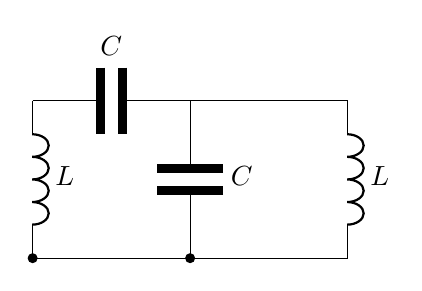
\begin{tikzpicture}[transform shape]
\ctikzset{label/align = smart}
\draw (0, 2) to [american inductor, l=$L$] (0, 0);
\draw (0, 2) to [capacitor, l=$C$, line width=1.5] (2, 2);
\draw (2, 2) to [capacitor, l=$C$, line width=1.5] (2, 0);
\draw (0, 0) -- (4, 0);
\draw (4, 2) to [american inductor, l=$L$] (4, 0);
\draw (4, 2) -- (2, 2);
\draw (0, 0) to [open, *-] (0, 2);
\draw (2, 0) to [open, *-] (0, 2);
\end{tikzpicture}
\end{center}
Note that for an inductor, the impedance is given by 
\[Z_L = i\omega L\]
while for a capacitor, the impedance is given by 
\[Z_C = \frac{1}{i\omega C}.\]
At resonance frequency, the impedance between the two points approaches zero. The impedance in the both temrinals will be given as 
\[Z = i\omega L + \frac{1}{i\omega C } + \frac{i\omega L \times 1/i\omega C}{i\omega L + 1/i\omega C}\to 0.\]
This is a quartic equation, and we find that upon algebraic manipulation that the answer is 
\[\omega = \frac{\sqrt{5} \pm 1}{2}\omega_0 = \frac{\sqrt{5} \pm 1}{2\sqrt{LC}}.\]
\tcbline
\textbf{Kirchoff's Laws}
\\
Let the charge on the first capacitor be $Q_1$ and the charge on the second capacitor be $Q_2$. The current flowing through both of these capacitors are $I_1$ and $I_2$ respectively, and therefore, the current flowing through the first inductor is $I_1$ and the current flowing through the second inductor is $I_1 - I_2$. 
\begin{center}
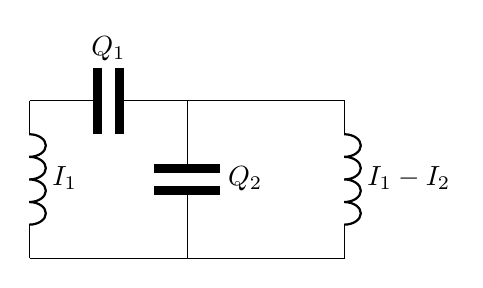
\begin{tikzpicture}[transform shape]
\ctikzset{label/align = smart}
\draw (0, 2) to [american inductor, l=$I_1$] (0, 0);
\draw (0, 2) to [capacitor, l=$Q_1$, line width=1.5] (2, 2);
\draw (2, 2) to [capacitor, l=$Q_2$, line width=1.5] (2, 0);
\draw (0, 0) -- (4, 0);
\draw (4, 2) to [american inductor, l=$I_1 - I_2$] (4, 0);
\draw (4, 2) -- (2, 2);
\end{tikzpicture}
\end{center}
By fact 2 (Kirchoff's Voltage Law), along a closed loop of an electrical circuit, the sum of voltage drops on the circuit elements (resistors, diodes, capacitors, etc) equals to the sum of the electromotive forces (of batteries and inductors). Mathematically,
\[\sum_{\text{wire forming a closed loop}} V_{\nu} = 0.\]
Therefore, by writing Kirchoff's Law on the first (leftmost) loop and the second (rightmost loop), we get these two equations:
\begin{align*}
\frac{Q_1}{C} + \frac{Q_2}{C} - L\dot{I}_1 &= 0 \\
-\frac{Q_2}{C} - L(\dot{I}_1 - \dot{I}_2) &= 0
\end{align*}
Note that $I_1 = \dot{Q}_1$ and $I_2 = \dot{Q}_2$. Substituting gives us 
\begin{align*}
\frac{Q_1}{C} + \frac{Q_2}{C} - L\ddot{Q}_1 &= 0 \\
-\frac{Q_2}{C} - L(\ddot{Q}_1 - \ddot{Q}_2) &= 0
\end{align*}
Rearranging the first equation by writing $\omega_0 = 1/\sqrt{LC}$ tells us 
\[\ddot{Q}_1 = \frac{Q_1}{LC} + \frac{Q_2}{LC}\implies \ddot{Q_1} = \omega_0^2 (Q_1 + Q_2).\]
We can similarly do the same thing for the second equation. First, we rearrange as shown below:
\[\ddot{Q}_1 - \ddot{Q_2} = -\frac{Q_2}{LC}\implies \ddot{Q}_1 - \ddot{Q_2} = -\omega_0^2 Q_2.\]
We then substitute our first equation into the second one to get 
\[ \omega_0^2 (Q_1 + Q_2) - \ddot{Q}_2 = -\omega_0^2 Q_2\implies \ddot{Q}_2 = \omega_0^2 (Q_1 + 2Q_2).\]
Regrouping both equations together gives us a pair of coupled differential equations:
\begin{align*}
\ddot{Q_1} &= \omega_0^2 (Q_1 + Q_2) \\
\ddot{Q}_2 &= \omega_0^2 (Q_1 + 2Q_2)
\end{align*}
Using the definition of a normal mode 
\[
\begin{pmatrix}
Q_1 \\
Q_2 
\end{pmatrix}
= 
\text{Re} \left[
\begin{pmatrix}
A_1 \\
A_2 
\end{pmatrix}
e^{i (\omega t + \phi)}
\right]
\]
we can then rearrange to find
$$\begin{aligned}
- \omega^{2}A_1 &= \omega_0^2 A_1 + \omega_0^2 A_2 & \Rightarrow\quad & 0=\left(\omega_0^2 + \omega^2 \right) A_{1}+ \omega_0^2 A_2 \\
-\omega^{2}A_2 &= \omega_0^2 A_1 + 2\omega_0^2 A_2 & \Rightarrow \quad & 0= \omega_0^2 A_1 + (2\omega_0^2 + \omega^2)A_2  
\end{aligned}$$
Now, rewrite in matrix format
\[
\begin{pmatrix}
\omega_0^2 + \omega^2 & \omega_0^2 \\
\omega_0^2 & 2\omega_0^2 + \omega^2 
\end{pmatrix}
\begin{pmatrix}
A_1 \\
A_2 
\end{pmatrix}
= 
0.\]
To get a solution we need to solve the equation where the determinant of the left matrix is zero
\[
\begin{vmatrix}
\omega_0^2 + \omega^2 & \omega_0^2 \\
\omega_0^2 & 2\omega_0^2 + \omega^2
\end{vmatrix}
=
0\]
This can be written as 
\[(\omega_0^2 + \omega^2)(2\omega_0^2 - \omega^2) - \omega_0^4 = 0.\]
By writing $\omega_0^2 \equiv \Omega$ and $\omega^2 \equiv \varphi$, we can solve this equation to find that 
\[\omega = \frac{\sqrt{5}\pm 1}{2}\omega_0 = \frac{\sqrt{5}\pm 1}{2\sqrt{LC}}.\]
\tcbline
\textbf{Using Lagrangian Method}
\\

Let the charge on the first capacitor be $Q_1$ and the charge on the second capacitor be $Q_2$. The current flowing through both of these capacitors are $I_1$ and $I_2$ respectively, and therefore, the current flowing through the first inductor is $I_1$ and the current flowing through the second inductor is $I_1 - I_2$. 
\begin{center}
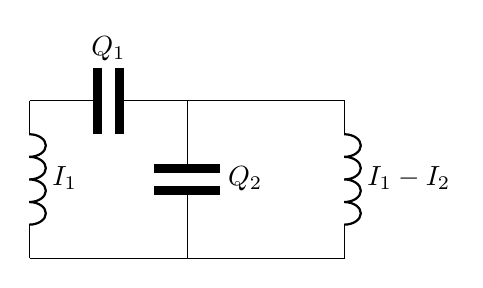
\begin{tikzpicture}[transform shape]
\ctikzset{label/align = smart}
\draw (0, 2) to [american inductor, l=$I_1$] (0, 0);
\draw (0, 2) to [capacitor, l=$Q_1$, line width=1.5] (2, 2);
\draw (2, 2) to [capacitor, l=$Q_2$, line width=1.5] (2, 0);
\draw (0, 0) -- (4, 0);
\draw (4, 2) to [american inductor, l=$I_1 - I_2$] (4, 0);
\draw (4, 2) -- (2, 2);
\end{tikzpicture}
\end{center}
Consider the energy of the system. For a capacitor, the potential energy is given as 
\[U = \frac{1}{2}CV^2 = \frac{1}{2}\frac{Q^2}{C}.\]
Therefore, the total potential energy is given as 
\[U_{\text{tot}} = \frac{1}{2}\frac{Q_1^2}{C} + \frac{1}{2}\frac{Q_2^2}{C}.\]
Note that in this problem, we take our generalized cooordinate to be the charge. We know that $I_1 = \dot{Q}_1$ and $I_2 = \dot{Q}_2$. We also know that the energy of an inductor is 
\[T = \frac{1}{2}LI^2 = \frac{1}{2}L\dot{Q}^2\]
and therefore, the total kinetic energy is 
\[T = \frac{1}{2}L\dot{Q}_1^2 + \frac{1}{2}L(\dot{Q}_1 - \dot{Q}_2)^2.\]
The lagrangian of the system is therefore, 
\[\mathcal{L} \equiv T - U = \frac{1}{2}L\dot{Q}_1^2 + \frac{1}{2}L(\dot{Q}_1^2 - 2\dot{Q}_1\dot{Q}_2 + \dot{Q}_2) - \frac{1}{2}\frac{Q_1^2}{C} - \frac{1}{2}\frac{Q_2^2}{C}.\]
We now use the Euler-Lagrange equations for both generalized coordinates $Q_1$ and $Q_2$.
\[\frac{d}{dt}\left(\frac{\partial\mathcal{L}}{\partial \dot{Q}_1}\right) \implies \frac{\partial \mathcal{L}}{\partial Q_1} = 2L\ddot{Q}_1 - L\ddot{Q}_2 = -\frac{Q_1}{C}\]and
\[\frac{d}{dt}\left(\frac{\partial\mathcal{L}}{\partial \dot{Q}_2}\right) = \frac{\partial \mathcal{L}}{\partial Q_2} \implies L\ddot{Q}_2 - L\ddot{Q}_1 = -\frac{Q_2}{C}.\]
Using the fact that $\omega_0 = 1/\sqrt{LC}$, we can rewrite our equations of motion to be 
\begin{align*}
2\ddot{Q}_1 - \ddot{Q}_2 &= -\omega_0^2 Q_1 \\
\ddot{Q}_2 - \ddot{Q}_1 &= -\omega_0^2 Q_2
\end{align*}
We can isolate the first equation to get the equation 
\[\ddot{Q}_2 = 2\ddot{Q}_1 + \omega_0^2 Q_1\]
which means upon substitution into the secpnd equation gives us 
\[2\ddot{Q}_1 + \omega_0^2 Q+1 - \ddot{Q}_1 = - \omega_0^2 Q_2\implies \ddot{Q}_1 = -\omega_0^2 (Q_1 + Q_2).\]
Similarly, we can now substitute this equation into equation the first equation to get 
\[\ddot{Q}_2 = -2\omega_0^2 (Q_1 + Q_2) + \omega_0^2 Q_1 = -\omega_0^2 (Q_1 + 2Q_2).\]
Putting these two equations together into a coupled differential equation gives us 
\begin{align*}
\ddot{Q}_1 &= -\omega_0^2 (Q_1 + Q_2) \\
\ddot{Q}_2 &= -\omega_0^2 (Q_1 + 2Q_2)
\end{align*}
Now, use the same approach as given in the Kirchoff's solution to get the given answer. 
\end{solution}
\input{100}
\input{101}
\input{102}
\input{103}
\input{104}
\begin{solution}{hard}
By idea 17, the circuit is evidently, self dual. Thus, let us draw a diagram of its dual circuit; the dual circuit is obtained by putting one node inside each face of the original circuit, and connecting the new nodes with wires so that each old wire is crossed by exactly one new wire, see below.
\begin{center}
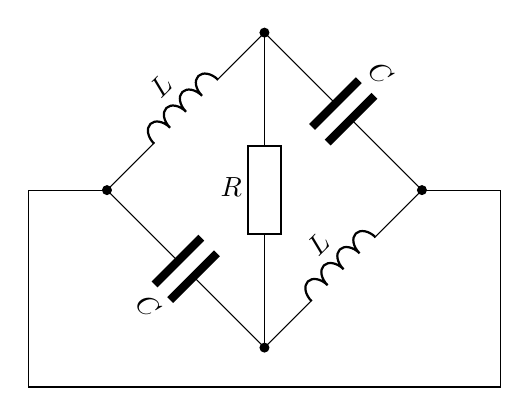
\begin{tikzpicture}[transform shape, scale=1.0]
\ctikzset{bipoles/thickness=2}
\ctikzset{label/align = smart}
\draw (4, 0) to [C=$C$, line width=1.5] (2, 2);
\draw (2, 2) to [inductor=$L$] (4, 4) to [C=$C$, line width=1.5] (6, 2);
\draw (4, 0) to [inductor=$L$] (6, 2);
\draw (4, 0) to [R=$R$, fill =white] (4,4);
\draw (2, 2) to [open, *-] (3, 2);
\draw (4, 4) to [open, *-] (5, 4);
\draw (4, 0) to [open, *-] (5, 4);
\draw (6, 2) to [open, *-] (5, 4);
\draw (2, 2) -- (1, 2) -- (1, -0.5);
\draw (6, 2) -- (7, 2) -- (7, -0.5);
\draw (1, -0.5) -- (7, -0.5);
\end{tikzpicture}
\qquad 
    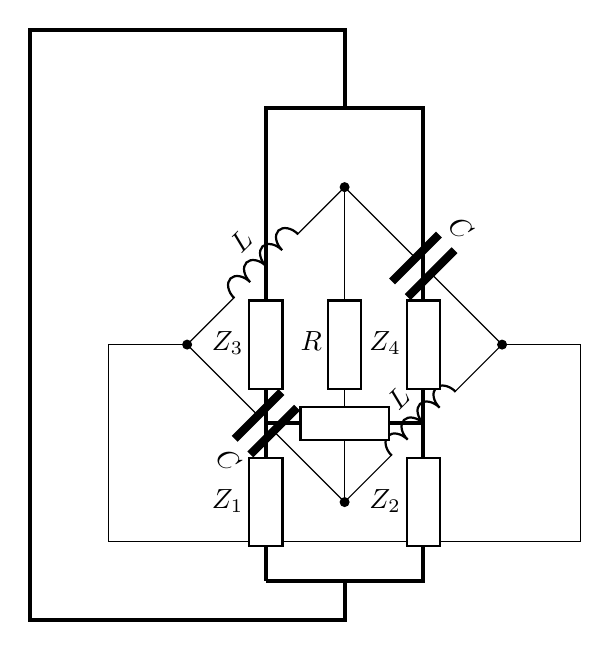
\begin{tikzpicture}[transform shape, scale=1.0]
\ctikzset{bipoles/thickness=2}
\ctikzset{label/align = smart}
\draw (4, 0) to [C=$C$, line width=1.5] (2, 2);
\draw (2, 2) to [inductor=$L$] (4, 4) to [C=$C$, line width=1.5] (6, 2);
\draw (4, 0) to [inductor=$L$] (6, 2);
\draw (4, 0) to [R=$R$, fill =white] (4,4);
\draw (2, 2) to [open, *-] (3, 2);
\draw (4, 4) to [open, *-] (5, 4);
\draw (4, 0) to [open, *-] (5, 4);
\draw (6, 2) to [open, *-] (5, 4);
\draw (2, 2) -- (1, 2) -- (1, -0.5);
\draw (6, 2) -- (7, 2) -- (7, -0.5);
\draw (1, -0.5) -- (7, -0.5);
\draw [line width=0.5mm] (3, -1) -- (3, 5) -- (5, 5) -- (5, -1) -- (3, -1);
\draw [line width=0.5mm] (4, -1) -- (4, -1.5) -- (0, -1.5) -- (0, 6) -- (4, 6) -- (4, 5);
\draw [line width=0.5mm] (3, 1) -- (5, 1);
\draw (3, -1) to [R=$Z_1$, fill=white] (3, 1);
\draw (5, -1) to [R=$Z_2$, fill=white] (5, 1);
\draw (3, 1) to [R=$Z_3$, fill=white] (3, 3);
\draw (5, 1) to [R=$Z_4$, fill=white] (5, 3);
\draw (3, 1) to [R, fill=white] (5, 1);
\end{tikzpicture}
\end{center}
Now, the complex impedances of each circuit component are $Z_C = \frac{1}{i\omega C}, Z_L = i\omega L, Z_R = \sqrt{\frac{L}{C}}$. We would obtain exactly the same set of equations if we were considering the new circuit as a usual resistor network with resistances being equal to the conductances of the old circuit. Multiplying each circuit component by the factor $\alpha = \frac{C}{L}$ preserves symmetry as $Z^{\prime}_C = \alpha Z_C = 1/i\omega L$, $Z^{\prime}_L = \alpha Z_L = i\omega C$, and $Z^{\prime}_R = \alpha Z_R = \sqrt{C/L}$ (thus the impedances are reciprocals of the original impedance, and symmetry among the circuit components are maintained). Since
the impedance is independent of the sinusoidal circular frequency $\omega$, it is equivalent to an active resistor.  Thus, the impedance of the original circuit can be described as 
\[Z\frac{C}{L} = \frac{1}{Z}\implies Z = \sqrt{\frac{L}{C}}\]
and hence, we can write 
\[V = IZ\implies I = V_0 \sqrt{\frac{C}{L}}.\]
\end{solution}
\input{106}
\begin{solution}{normal}
Let us denote the node $\text{O}$ to be where the resistor of resistance $R_2$ and inductor of inductance $L_1$ meet. Similarly, let us label the node $\text{C}$ to be where the resistor $R_1$ and inductor $L_2$ meet. We can use similar reasoning to conclude that $V_{OB}\perp V_{BC}$. Note that inductors lead the current by $\pi/2$ degrees while resistors have neither lag nor lead. This means that when drawing a voltage phasor, $V_{OA}$ is orthogonal to $V_{AC}$. Since there is a phase shift $\varphi$ between currents through nodes $\text{A}$ and $\text{B}$, then we can say that $\angle ABC = \varphi$. We can then inscribe the vectors inside a circle $\Gamma$ as shown below:
\begin{center}
\begin{asy}
import olympiad;
size(7cm);
pair A = dir(80);
pair B = dir(180);
pair C = dir(360);

pair X = dir(250);
pair Y = dir(40);
filldraw(unitcircle, opacity(0.1)+lightblue, lightblue);
fill(A--B--C--cycle, opacity(0.1)+mediumcyan);

fill(B--X--C--cycle, opacity(0.1)+mediumcyan);

markscalefactor = 0.02;
draw(anglemark(C, B, A));
markscalefactor = 0.025;
draw(anglemark(X, B, C));

draw(A--X, heavycyan);

pair O = origin;
draw(A--O, heavygreen);
draw(anglemark(C, O, A));
markscalefactor = 0.02;
draw(anglemark(C, X, A));

pair I = extension(A, X, B, Y);

draw(B--C, arrow=Arrow(8));
draw(B--A, blue, arrow=Arrow(8));
draw(B--C, arrow=Arrow(8));
draw(A--C, purple, arrow=Arrow(8));
draw(B--X, purple, arrow=Arrow(8));
draw(X--C, blue, arrow=Arrow(8));

dot("$A$", A, dir(A));
dot("$O$", B, dir(B));
dot("$C$", C, dir(C));
dot("$B$", X, dir(X));
dot("$D$", O, dir(315));
\end{asy}
\end{center}
\noindent \textbf{(a)} In $\Delta OAC$, $AD$ is the median to the hypotenuse and by Thale's theorem, it is half the length of $OC$. Since $OC = V_0$, this means that $AD = V_0/2$. 
\vspace{3mm}

\noindent \textbf{(b)} Since $\angle CBA = \varphi$, we then can say by inscribed angle theorem that $\angle CDA = 2\varphi$ which is the phase shift between $V_{AD}$ and $V_{DB}$.
\end{solution}
\begin{solution}{normal}
According to idea 52, we draw a phasor diagram of the circuit. The current $I$ through the circuit components remains the same through all the components. By idea 44, the voltage in the circuit will be $V = IZ$ where $Z$ is the circuit's complex impedance. First, we note that the impedance of a capacitor is given as 
\[Z_C = \frac{1}{i\omega C}\]
while the impedance of an inductor is given as 
\[Z_L = i\omega L.\]
For a resistor of resistance $R$, the impedance is the same as it's regular resistance $Z_R = R$. Second, note that current and voltage have no lag or lead in terms of resistors. 
\vspace{3mm}

\noindent Let us write that $A$ is the node between the inductor $L_1$ and the resistor $R_1$ while $B$ is the node between the capacitor $C$ and the resistor $R_2$. 
\vspace{3mm}

\begin{center}
\begin{asy}
import olympiad;
size(7cm);
pair A = dir(80);
pair B = dir(180);
pair C = dir(360);

pair X = dir(250);
pair Y = dir(40);
draw(B--A, blue, arrow=Arrow(8));
draw(B--C, arrow=Arrow(8));
draw(A--C, purple, arrow=Arrow(8));

draw(B--X, heavygreen, arrow=Arrow(8));
draw(X--C, purple, arrow=Arrow(8));

markscalefactor = 0.02;
draw(anglemark(C, B, A));
markscalefactor = 0.025;
draw(anglemark(X, B, C));
label("$\frac{\pi}{2} - \varphi$", (-0.6, 0), N);

draw(A--X, heavycyan);

pair O = origin;

pair I = extension(A, X, B, Y);

dot("$A$", A, dir(A));
dot("$O$", B, dir(B));
dot("$C$", C, dir(C));
dot("$B$", X, dir(X));
\end{asy}
\end{center}
In the problem, it says the phase shift between the inductor current and the input voltage is $\varphi$. We know that an inductor voltage leads the current by $\pi/2$ radians which means that the phase between the inductor voltage and input voltage is $\pi/2 + \varphi$ radians. Graphically, we can represent the phasor of the inductor $L_1$ with the blue vector shown in the figure below and write that $\angle AOC = \pi/2 - \varphi$ since $\angle AOC$ has to be acute which implies that the phase is negative. 
\vspace{3mm}

\noindent Let us represent the phasor of the capacitor as the green vector. We note that it's impedance is negative since the complex voltage amplitude is $I/i\omega C$ which rotates the vector clockwise. 
\vspace{3mm}

\noindent Similarly, the current through $R_1$ is the same as $L$ and the current through $R_2$ is the same as $C$. There is no lead/lag through these resistors but there is lag of $\pi/2$ in the inductor and a lead of $\pi/2$ in the capacitor which allows us to combine them together as shown below with the two purple arrows. We can now inscribe these phasors into a circle $\Gamma$ as shown below. 
\begin{center}
\begin{asy}
import olympiad;
size(7cm);
pair A = dir(80);
pair B = dir(180);
pair C = dir(360);

pair X = dir(250);
pair Y = dir(40);
filldraw(unitcircle, opacity(0.1)+lightblue, lightblue);
fill(A--B--C--cycle, opacity(0.1)+mediumcyan);

fill(B--X--C--cycle, opacity(0.1)+mediumcyan);

markscalefactor = 0.02;
draw(anglemark(C, B, A));
markscalefactor = 0.025;
draw(anglemark(X, B, C));
label("$\frac{\pi}{2} - \varphi$", (-0.6, 0), N);

draw(A--X, heavycyan);

pair O = origin;

pair I = extension(A, X, B, Y);

draw(B--C, arrow=Arrow(8));
draw(B--A, blue, arrow=Arrow(8));
draw(B--C, arrow=Arrow(8));
draw(A--C, purple, arrow=Arrow(8));
draw(B--X, heavygreen, arrow=Arrow(8));
draw(X--C, purple, arrow=Arrow(8));

dot("$A$", A, dir(A));
dot("$O$", B, dir(B));
dot("$C$", C, dir(C));
dot("$B$", X, dir(X));
dot("$\Gamma$", O, dir(315));
\end{asy}
\end{center}
Now, finally note that we want to find $\angle ABO$. Since $\angle AOC = \pi/2 - \varphi$, this means that $\angle ACO = \varphi$ and since arc $\overset{\large\frown}{OA}$ is subtended by the same angles $\angle ABO$ and $\angle ACO$, we can say that $\angle ABO = \angle ACO = \varphi$.

\end{solution}
\input{109}
\input{110}
\begin{solution}{hard}

\end{solution}

\end{document}